\begin{figure}
\begin{center}
    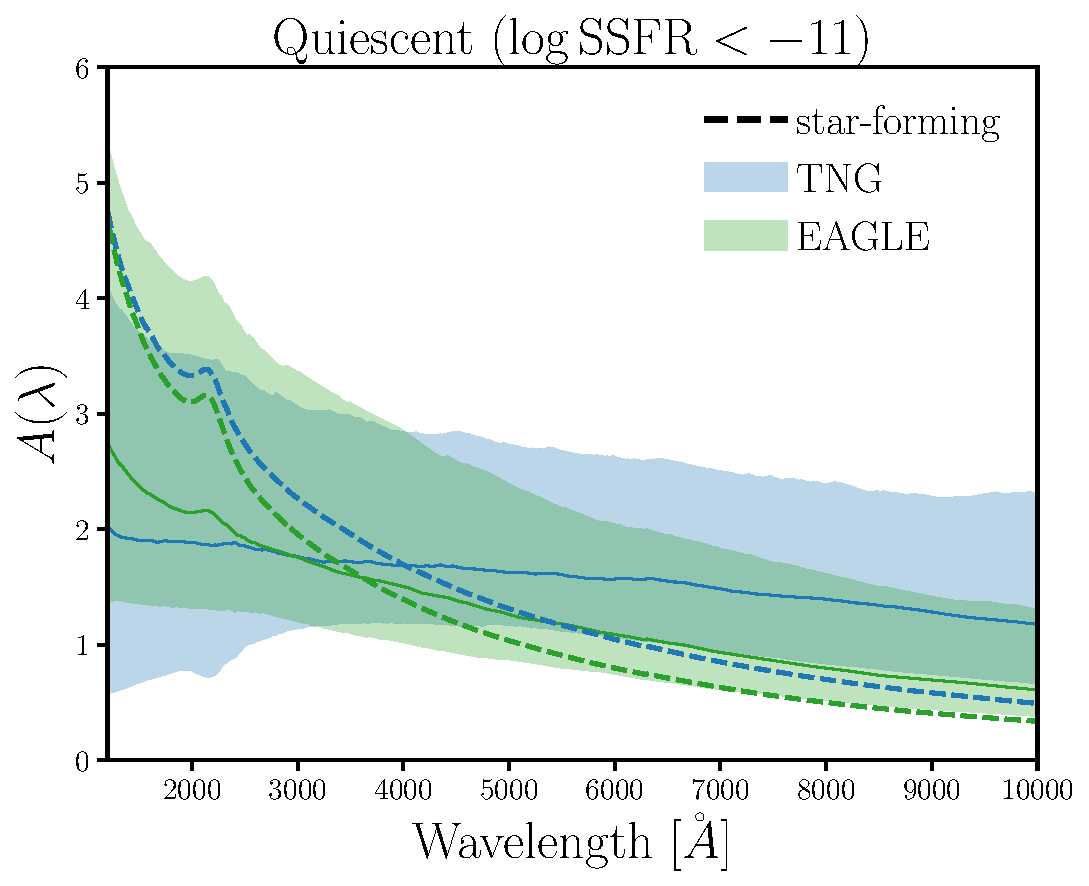
\includegraphics[width=0.5\textwidth]{figs/abc_q_atten_unnorm.pdf}
    \caption{\label{fig:q_raw_atten}
    \chedit{
        The attenuation curves of quiescent galaxies predicted by the \eda~for
        median posterior parameter values of TNG (blue) and EAGLE (green).
        Galaxies are classified as quiescent using a $\log \ssfr < -11~yr^{-1}$
        cut.
        We mark the $1\sigma$ standard deviation of the attenuation curves with
        the shaded region and include the predicted attenuation curves of
        star-forming galaxies for comparison (dashed). 
        For both TNG and EAGLE, \emph{the \eda~predicts significant UV and
        optical dust attenuation in quiescent galaxies with an overall shallow
        attenuation curve}.
    }
    }
\end{center}
\end{figure}
\subsection{The Attenuation Curves of Quiescent Galaxies}  
\chedit{
    We have demonstrated so far that the \eda~can reproduce the observed UV and
    optical color-magnitude relations.  
    In doing so, it also predicts attenuation-slope relation and dust
    attenuation curves of star-forming galaxies that are in good agreement with
    observations and radiative transfer simulations. 
    Beyond reproducing previous work, the \eda~also makes predictions on the dust
    attenuation of quiescent galaxies, which is still poorly constrained by
    obsevations. 
    There are many challenges to measuring the attenuation curves of quiescent galaxies directly from observations.
    Methods that rely on IR luminosities can be contaminated by MIR emission
    from AGN heating nearby dust~\citep{kirkpatrick2015}. 
    SED fitting methods must also account for AGN MIR
    emission~\citep{salim2016, leja2018, salim2018} and struggle to tightly
    constrain dust attenuation for quiescent galaxies due to the degeneracies
    with star formation history and metallicity.
}

With a forward modeling approach, we circumvent these challenges. 
Instead, we derive the attenuation curves necessary for the simulated quiescent population to reproduce the observed optical and UV photometry. 
\chedit{
    In Figure~\ref{fig:q_raw_atten}, we present the attenuation curves of
    quiescent galaxies predicted by the \eda~for the median posterior parameter
    values of TNG (blue) and EAGLE (green). 
    Quiescent galaxies are classified using a $\log\ssfr < -11~{yr}^{-1}$ cut. 
    Unlike Figure~\ref{fig:sfatten}, the attenuation curves are \emph{not}
    normalized at $3000\AA$. 
    For comparison, we include $A(\lambda)$ of star-forming galaxies predicted
    by the \eda~(dotted).
    Both TNG+\eda~and EAGLE+\eda predict significant dust attenuation in
    quiescent galaxies: $A(\lambda) \gtrsim 1$ throughout the UV and optical. 
    Their attenuation curves are also significantly shallower than the
    attenuation curves of star-forming galaxies. 
}


\chedit{
    The quiescent galaxy dust attenuation we predict is not a consequence of
    the parameterization of our \eda~prescription. 
    Without dust both TNG and EAGLE predict quiescent galaxies that are too
    luminous and bluer in the optical than SDSS observations (Figure~\ref{fig:obs}). 
    Therefore, to match the SDSS color-magnitude relations, significant
    attenuation is necessary to lower their luminosities but with a shallow
    slope that reddens their $\gr$ colors while maintaining their $\fnuv$ colors.
    This is also the reason why TNG has a shallower slope than EAGLE: without
    dust, TNG has a quiescent population that is redder in both UV and optical.   
}

\chedit{    
    Dust attenuation in quiescent galaxies, which is typically neglected, has
    significant implications.  
    For instance, it strengthens the evidence for the UV upturn phenomenon, the
    unexpected detections of UV flux in quiescent galaxies~\citep[\eg][]{code1969,
    oconnell1999, lecras2016, ali2018, dantas2021}. 
    Better constraints on the attenuation in quiescent galaxies may help
    discern among the different hypotheses: residual star formation activity~\citep[\eg~][]{kaviraj2007}, post-main-sequence stellar
    evolutionary phases~\citep[\eg~][]{yi1997}, or binary systems~\citep[\eg~][]{han2007}.
    Since the attenuation curves of quiescent galaxies are difficult to measure
    from observations, the \eda~predictions highlight the advantages of a
    forward modeling approach and its complementarity with standard approaches. 
    We, however, note that since we only vary the \eda~parameters in our forward
    model, we do not explore whether the discrepancy between the quiescent
    populations in simulations and observations is due to shortcomings of the
    galaxy formation models. 
    In principle, and in future work, we can vary both the \eda~parameters and
    the parameters of the galaxy formation models and infer them simultaneously
    with a foward modeling approach. 
}
